\documentclass[twoside]{book}

% Packages required by doxygen
\usepackage{fixltx2e}
\usepackage{calc}
\usepackage{doxygen}
\usepackage[export]{adjustbox} % also loads graphicx
\usepackage{graphicx}
\usepackage[utf8]{inputenc}
\usepackage{makeidx}
\usepackage{multicol}
\usepackage{multirow}
\PassOptionsToPackage{warn}{textcomp}
\usepackage{textcomp}
\usepackage[nointegrals]{wasysym}
\usepackage[table]{xcolor}

% Font selection
\usepackage[T1]{fontenc}
\usepackage[scaled=.90]{helvet}
\usepackage{courier}
\usepackage{amssymb}
\usepackage{sectsty}
\renewcommand{\familydefault}{\sfdefault}
\allsectionsfont{%
  \fontseries{bc}\selectfont%
  \color{darkgray}%
}
\renewcommand{\DoxyLabelFont}{%
  \fontseries{bc}\selectfont%
  \color{darkgray}%
}
\newcommand{\+}{\discretionary{\mbox{\scriptsize$\hookleftarrow$}}{}{}}

% Page & text layout
\usepackage{geometry}
\geometry{%
  a4paper,%
  top=2.5cm,%
  bottom=2.5cm,%
  left=2.5cm,%
  right=2.5cm%
}
\tolerance=750
\hfuzz=15pt
\hbadness=750
\setlength{\emergencystretch}{15pt}
\setlength{\parindent}{0cm}
\setlength{\parskip}{0.2cm}
\makeatletter
\renewcommand{\paragraph}{%
  \@startsection{paragraph}{4}{0ex}{-1.0ex}{1.0ex}{%
    \normalfont\normalsize\bfseries\SS@parafont%
  }%
}
\renewcommand{\subparagraph}{%
  \@startsection{subparagraph}{5}{0ex}{-1.0ex}{1.0ex}{%
    \normalfont\normalsize\bfseries\SS@subparafont%
  }%
}
\makeatother

% Headers & footers
\usepackage{fancyhdr}
\pagestyle{fancyplain}
\fancyhead[LE]{\fancyplain{}{\bfseries\thepage}}
\fancyhead[CE]{\fancyplain{}{}}
\fancyhead[RE]{\fancyplain{}{\bfseries\leftmark}}
\fancyhead[LO]{\fancyplain{}{\bfseries\rightmark}}
\fancyhead[CO]{\fancyplain{}{}}
\fancyhead[RO]{\fancyplain{}{\bfseries\thepage}}
\fancyfoot[LE]{\fancyplain{}{}}
\fancyfoot[CE]{\fancyplain{}{}}
\fancyfoot[RE]{\fancyplain{}{\bfseries\scriptsize Generated on Thu Apr 23 2015 14\+:45\+:32 for Booklook Crawlers by Doxygen }}
\fancyfoot[LO]{\fancyplain{}{\bfseries\scriptsize Generated on Thu Apr 23 2015 14\+:45\+:32 for Booklook Crawlers by Doxygen }}
\fancyfoot[CO]{\fancyplain{}{}}
\fancyfoot[RO]{\fancyplain{}{}}
\renewcommand{\footrulewidth}{0.4pt}
\renewcommand{\chaptermark}[1]{%
  \markboth{#1}{}%
}
\renewcommand{\sectionmark}[1]{%
  \markright{\thesection\ #1}%
}

% Indices & bibliography
\usepackage{natbib}
\usepackage[titles]{tocloft}
\setcounter{tocdepth}{3}
\setcounter{secnumdepth}{5}
\makeindex

% Hyperlinks (required, but should be loaded last)
\usepackage{ifpdf}
\ifpdf
  \usepackage[pdftex,pagebackref=true]{hyperref}
\else
  \usepackage[ps2pdf,pagebackref=true]{hyperref}
\fi
\hypersetup{%
  colorlinks=true,%
  linkcolor=blue,%
  citecolor=blue,%
  unicode%
}

% Custom commands
\newcommand{\clearemptydoublepage}{%
  \newpage{\pagestyle{empty}\cleardoublepage}%
}


%===== C O N T E N T S =====

\begin{document}

% Titlepage & ToC
\hypersetup{pageanchor=false,
             bookmarks=true,
             bookmarksnumbered=true,
             pdfencoding=unicode
            }
\pagenumbering{roman}
\begin{titlepage}
\vspace*{7cm}
\begin{center}%
{\Large Booklook Crawlers \\[1ex]\large 0.\+9 }\\
\vspace*{1cm}
{\large Generated by Doxygen 1.8.9.1}\\
\vspace*{0.5cm}
{\small Thu Apr 23 2015 14:45:32}\\
\end{center}
\end{titlepage}
\clearemptydoublepage
\tableofcontents
\clearemptydoublepage
\pagenumbering{arabic}
\hypersetup{pageanchor=true}

%--- Begin generated contents ---
\chapter{Hierarchical Index}
\section{Class Hierarchy}
This inheritance list is sorted roughly, but not completely, alphabetically\+:\begin{DoxyCompactList}
\item \contentsline{section}{bookcrawl.\+assigner.\+Book\+Assigner}{\pageref{classbookcrawl_1_1assigner_1_1BookAssigner}}{}
\item Item\begin{DoxyCompactList}
\item \contentsline{section}{bookcrawl.\+items.\+Amazon\+Page\+Item}{\pageref{classbookcrawl_1_1items_1_1AmazonPageItem}}{}
\item \contentsline{section}{bookcrawl.\+items.\+Amazon\+Search\+Item}{\pageref{classbookcrawl_1_1items_1_1AmazonSearchItem}}{}
\item \contentsline{section}{bookcrawl.\+items.\+Bookcrawl\+Item}{\pageref{classbookcrawl_1_1items_1_1BookcrawlItem}}{}
\end{DoxyCompactList}
\item object\begin{DoxyCompactList}
\item \contentsline{section}{bookcrawl.\+pipelines.\+Bookcrawl\+Pipeline}{\pageref{classbookcrawl_1_1pipelines_1_1BookcrawlPipeline}}{}
\end{DoxyCompactList}
\end{DoxyCompactList}

\chapter{Class Index}
\section{Class List}
Here are the classes, structs, unions and interfaces with brief descriptions\+:\begin{DoxyCompactList}
\item\contentsline{section}{\hyperlink{classbookcrawl_1_1items_1_1AmazonPageItem}{bookcrawl.\+items.\+Amazon\+Page\+Item} }{\pageref{classbookcrawl_1_1items_1_1AmazonPageItem}}{}
\item\contentsline{section}{\hyperlink{classbookcrawl_1_1items_1_1AmazonSearchItem}{bookcrawl.\+items.\+Amazon\+Search\+Item} }{\pageref{classbookcrawl_1_1items_1_1AmazonSearchItem}}{}
\item\contentsline{section}{\hyperlink{classbookcrawl_1_1assigner_1_1BookAssigner}{bookcrawl.\+assigner.\+Book\+Assigner} }{\pageref{classbookcrawl_1_1assigner_1_1BookAssigner}}{}
\item\contentsline{section}{\hyperlink{classbookcrawl_1_1items_1_1BookcrawlItem}{bookcrawl.\+items.\+Bookcrawl\+Item} }{\pageref{classbookcrawl_1_1items_1_1BookcrawlItem}}{}
\item\contentsline{section}{\hyperlink{classbookcrawl_1_1pipelines_1_1BookcrawlPipeline}{bookcrawl.\+pipelines.\+Bookcrawl\+Pipeline} }{\pageref{classbookcrawl_1_1pipelines_1_1BookcrawlPipeline}}{}
\end{DoxyCompactList}

\chapter{Class Documentation}
\hypertarget{classbookcrawl_1_1items_1_1AmazonPageItem}{}\section{bookcrawl.\+items.\+Amazon\+Page\+Item Class Reference}
\label{classbookcrawl_1_1items_1_1AmazonPageItem}\index{bookcrawl.\+items.\+Amazon\+Page\+Item@{bookcrawl.\+items.\+Amazon\+Page\+Item}}
Inheritance diagram for bookcrawl.\+items.\+Amazon\+Page\+Item\+:\begin{figure}[H]
\begin{center}
\leavevmode
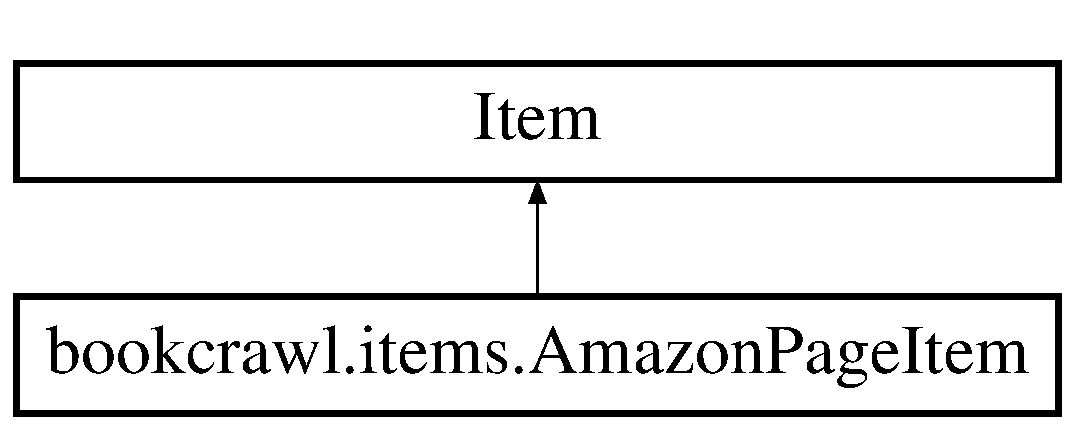
\includegraphics[height=2.000000cm]{classbookcrawl_1_1items_1_1AmazonPageItem}
\end{center}
\end{figure}
\subsection*{Static Public Attributes}
\begin{DoxyCompactItemize}
\item 
\hypertarget{classbookcrawl_1_1items_1_1AmazonPageItem_a7381e478950d2ba174ccc7c902a7f7fe}{}tuple {\bfseries p\+\_\+title} = scrapy.\+Field()\label{classbookcrawl_1_1items_1_1AmazonPageItem_a7381e478950d2ba174ccc7c902a7f7fe}

\item 
\hypertarget{classbookcrawl_1_1items_1_1AmazonPageItem_a55a509fe9e5f3751689d47ee84afb10e}{}tuple {\bfseries p\+\_\+author} = scrapy.\+Field()\label{classbookcrawl_1_1items_1_1AmazonPageItem_a55a509fe9e5f3751689d47ee84afb10e}

\item 
\hypertarget{classbookcrawl_1_1items_1_1AmazonPageItem_a510f90f21779b357829320f6109655d4}{}tuple {\bfseries p\+\_\+pages} = scrapy.\+Field()\label{classbookcrawl_1_1items_1_1AmazonPageItem_a510f90f21779b357829320f6109655d4}

\end{DoxyCompactItemize}


\subsection{Detailed Description}
\begin{DoxyVerb}Part of a trio of objects designed to have data passed to
by the appropriate spider. Their fields are flushed to
a JSON-formatted file when their jobs are complete.

This item is associated with the BookSpider.
\end{DoxyVerb}
 

The documentation for this class was generated from the following file\+:\begin{DoxyCompactItemize}
\item 
items.\+py\end{DoxyCompactItemize}

\hypertarget{classbookcrawl_1_1items_1_1AmazonSearchItem}{}\section{bookcrawl.\+items.\+Amazon\+Search\+Item Class Reference}
\label{classbookcrawl_1_1items_1_1AmazonSearchItem}\index{bookcrawl.\+items.\+Amazon\+Search\+Item@{bookcrawl.\+items.\+Amazon\+Search\+Item}}
Inheritance diagram for bookcrawl.\+items.\+Amazon\+Search\+Item\+:\begin{figure}[H]
\begin{center}
\leavevmode
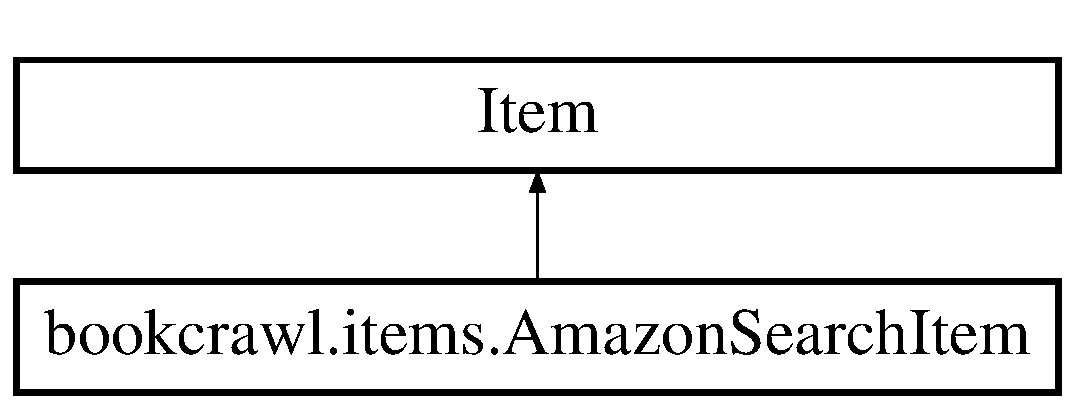
\includegraphics[height=2.000000cm]{classbookcrawl_1_1items_1_1AmazonSearchItem}
\end{center}
\end{figure}
\subsection*{Static Public Attributes}
\begin{DoxyCompactItemize}
\item 
\hypertarget{classbookcrawl_1_1items_1_1AmazonSearchItem_af9930b289b228a244fe6632015da26fd}{}tuple {\bfseries s\+\_\+title} = scrapy.\+Field()\label{classbookcrawl_1_1items_1_1AmazonSearchItem_af9930b289b228a244fe6632015da26fd}

\item 
\hypertarget{classbookcrawl_1_1items_1_1AmazonSearchItem_a4765956fc47e581851e5ad70917c1773}{}tuple {\bfseries s\+\_\+url} = scrapy.\+Field()\label{classbookcrawl_1_1items_1_1AmazonSearchItem_a4765956fc47e581851e5ad70917c1773}

\end{DoxyCompactItemize}


\subsection{Detailed Description}
\begin{DoxyVerb}Part of a trio of objects designed to have data passed to
by the appropriate spider. Their fields are flushed to
a JSON-formatted file when their jobs are complete.

This item is associated with the AmazonSpider.
\end{DoxyVerb}
 

The documentation for this class was generated from the following file\+:\begin{DoxyCompactItemize}
\item 
items.\+py\end{DoxyCompactItemize}

\hypertarget{classbookcrawl_1_1assigner_1_1BookAssigner}{}\section{bookcrawl.\+assigner.\+Book\+Assigner Class Reference}
\label{classbookcrawl_1_1assigner_1_1BookAssigner}\index{bookcrawl.\+assigner.\+Book\+Assigner@{bookcrawl.\+assigner.\+Book\+Assigner}}
\subsection*{Public Member Functions}
\begin{DoxyCompactItemize}
\item 
\hypertarget{classbookcrawl_1_1assigner_1_1BookAssigner_aa6bd54e63fb081f00f9d2e198cf51d96}{}def {\bfseries \+\_\+\+\_\+init\+\_\+\+\_\+} (self, path\+\_\+to\+\_\+page\+\_\+file, path\+\_\+to\+\_\+auth\+\_\+title\+\_\+file)\label{classbookcrawl_1_1assigner_1_1BookAssigner_aa6bd54e63fb081f00f9d2e198cf51d96}

\item 
\hypertarget{classbookcrawl_1_1assigner_1_1BookAssigner_a5043dcb507d28c5e1765e59cdca8e77d}{}def {\bfseries assignment\+\_\+iterator} (self)\label{classbookcrawl_1_1assigner_1_1BookAssigner_a5043dcb507d28c5e1765e59cdca8e77d}

\end{DoxyCompactItemize}
\subsection*{Public Attributes}
\begin{DoxyCompactItemize}
\item 
\hypertarget{classbookcrawl_1_1assigner_1_1BookAssigner_a0894529393c51c49ec698f308f75a241}{}{\bfseries page\+\_\+path}\label{classbookcrawl_1_1assigner_1_1BookAssigner_a0894529393c51c49ec698f308f75a241}

\item 
\hypertarget{classbookcrawl_1_1assigner_1_1BookAssigner_a680a55018bf04f6a99f5e5b7ee53d591}{}{\bfseries title\+\_\+path}\label{classbookcrawl_1_1assigner_1_1BookAssigner_a680a55018bf04f6a99f5e5b7ee53d591}

\end{DoxyCompactItemize}
\subsection*{Static Public Attributes}
\begin{DoxyCompactItemize}
\item 
\hypertarget{classbookcrawl_1_1assigner_1_1BookAssigner_ad9cfd3fde6448963e11ddc39613fe49e}{}string {\bfseries page\+\_\+path} = \char`\"{}\char`\"{}\label{classbookcrawl_1_1assigner_1_1BookAssigner_ad9cfd3fde6448963e11ddc39613fe49e}

\item 
\hypertarget{classbookcrawl_1_1assigner_1_1BookAssigner_a92af68d62f50eac5f4a844b137ae81a9}{}string {\bfseries title\+\_\+path} = \char`\"{}\char`\"{}\label{classbookcrawl_1_1assigner_1_1BookAssigner_a92af68d62f50eac5f4a844b137ae81a9}

\item 
\hypertarget{classbookcrawl_1_1assigner_1_1BookAssigner_ab7c26a5e57783fedebe46ec0629dcbf7}{}{\bfseries assign\+\_\+file} = None\label{classbookcrawl_1_1assigner_1_1BookAssigner_ab7c26a5e57783fedebe46ec0629dcbf7}

\item 
\hypertarget{classbookcrawl_1_1assigner_1_1BookAssigner_a110393458b3363cead5e74d3dd46b36b}{}tuple {\bfseries assignments} = Queue.\+Queue()\label{classbookcrawl_1_1assigner_1_1BookAssigner_a110393458b3363cead5e74d3dd46b36b}

\item 
\hypertarget{classbookcrawl_1_1assigner_1_1BookAssigner_a05cb03e8f88c29921d50eb2f5b30bde6}{}tuple {\bfseries jsondata} = json.\+load(self.\+assign\+\_\+file)\label{classbookcrawl_1_1assigner_1_1BookAssigner_a05cb03e8f88c29921d50eb2f5b30bde6}

\end{DoxyCompactItemize}


The documentation for this class was generated from the following file\+:\begin{DoxyCompactItemize}
\item 
assigner.\+py\end{DoxyCompactItemize}

\hypertarget{classbookcrawl_1_1items_1_1BookcrawlItem}{}\section{bookcrawl.\+items.\+Bookcrawl\+Item Class Reference}
\label{classbookcrawl_1_1items_1_1BookcrawlItem}\index{bookcrawl.\+items.\+Bookcrawl\+Item@{bookcrawl.\+items.\+Bookcrawl\+Item}}
Inheritance diagram for bookcrawl.\+items.\+Bookcrawl\+Item\+:\begin{figure}[H]
\begin{center}
\leavevmode
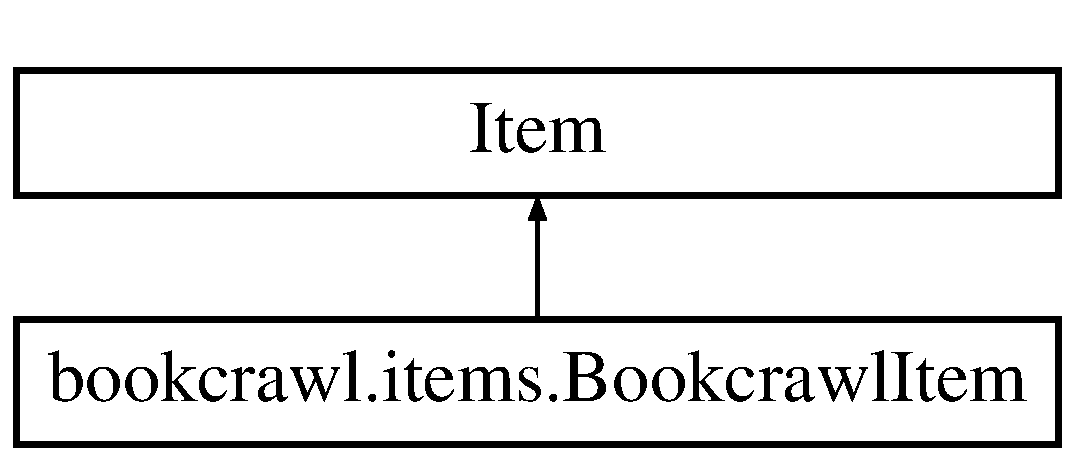
\includegraphics[height=2.000000cm]{classbookcrawl_1_1items_1_1BookcrawlItem}
\end{center}
\end{figure}
\subsection*{Static Public Attributes}
\begin{DoxyCompactItemize}
\item 
\hypertarget{classbookcrawl_1_1items_1_1BookcrawlItem_a037515234b6049bd0775a0a7356ffed2}{}tuple {\bfseries title} = scrapy.\+Field()\label{classbookcrawl_1_1items_1_1BookcrawlItem_a037515234b6049bd0775a0a7356ffed2}

\item 
\hypertarget{classbookcrawl_1_1items_1_1BookcrawlItem_ad2aafe952f2b7f9456890bd732439e41}{}tuple {\bfseries url} = scrapy.\+Field()\label{classbookcrawl_1_1items_1_1BookcrawlItem_ad2aafe952f2b7f9456890bd732439e41}

\item 
\hypertarget{classbookcrawl_1_1items_1_1BookcrawlItem_a68976a4d2435a542a155171412100961}{}tuple {\bfseries pages} = scrapy.\+Field()\label{classbookcrawl_1_1items_1_1BookcrawlItem_a68976a4d2435a542a155171412100961}

\item 
\hypertarget{classbookcrawl_1_1items_1_1BookcrawlItem_a903ec34de2f892101a57bcc499070add}{}tuple {\bfseries author} = scrapy.\+Field()\label{classbookcrawl_1_1items_1_1BookcrawlItem_a903ec34de2f892101a57bcc499070add}

\end{DoxyCompactItemize}


\subsection{Detailed Description}
\begin{DoxyVerb}Part of a trio of objects designed to have data passed to
by the appropriate spider. Their fields are flushed to
a JSON-formatted file when their jobs are complete.

This item is associated with the BookSpider.
\end{DoxyVerb}
 

The documentation for this class was generated from the following file\+:\begin{DoxyCompactItemize}
\item 
items.\+py\end{DoxyCompactItemize}

\hypertarget{classbookcrawl_1_1pipelines_1_1BookcrawlPipeline}{}\section{bookcrawl.\+pipelines.\+Bookcrawl\+Pipeline Class Reference}
\label{classbookcrawl_1_1pipelines_1_1BookcrawlPipeline}\index{bookcrawl.\+pipelines.\+Bookcrawl\+Pipeline@{bookcrawl.\+pipelines.\+Bookcrawl\+Pipeline}}
Inheritance diagram for bookcrawl.\+pipelines.\+Bookcrawl\+Pipeline\+:\begin{figure}[H]
\begin{center}
\leavevmode
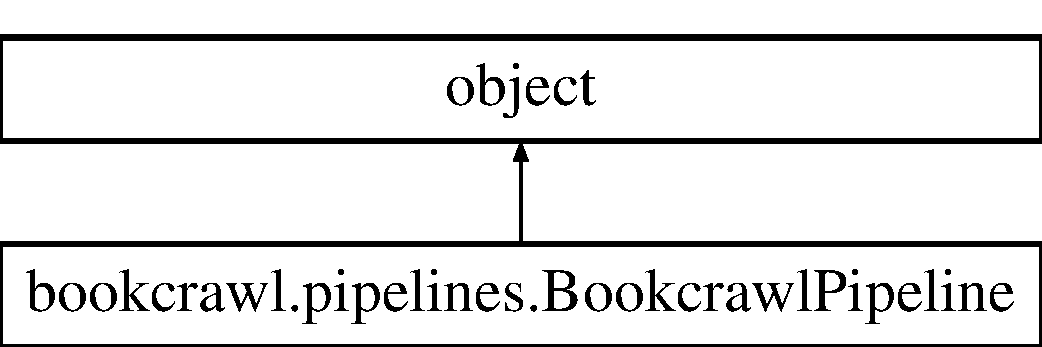
\includegraphics[height=2.000000cm]{classbookcrawl_1_1pipelines_1_1BookcrawlPipeline}
\end{center}
\end{figure}
\subsection*{Public Member Functions}
\begin{DoxyCompactItemize}
\item 
\hypertarget{classbookcrawl_1_1pipelines_1_1BookcrawlPipeline_ab383d9e621c958cebf999513fb63b0be}{}def {\bfseries \+\_\+\+\_\+init\+\_\+\+\_\+} (self)\label{classbookcrawl_1_1pipelines_1_1BookcrawlPipeline_ab383d9e621c958cebf999513fb63b0be}

\item 
\hypertarget{classbookcrawl_1_1pipelines_1_1BookcrawlPipeline_adca620f961c219e482251a9876067f77}{}def {\bfseries spider\+\_\+opened} (self, spider)\label{classbookcrawl_1_1pipelines_1_1BookcrawlPipeline_adca620f961c219e482251a9876067f77}

\item 
\hypertarget{classbookcrawl_1_1pipelines_1_1BookcrawlPipeline_a8ab0b673efe237450b816dd5ed693691}{}def {\bfseries spider\+\_\+closed} (self, spider)\label{classbookcrawl_1_1pipelines_1_1BookcrawlPipeline_a8ab0b673efe237450b816dd5ed693691}

\item 
\hypertarget{classbookcrawl_1_1pipelines_1_1BookcrawlPipeline_ac00ce6ac454846864e9ad549d1a55c28}{}def {\bfseries process\+\_\+item} (self, item, spider)\label{classbookcrawl_1_1pipelines_1_1BookcrawlPipeline_ac00ce6ac454846864e9ad549d1a55c28}

\end{DoxyCompactItemize}
\subsection*{Public Attributes}
\begin{DoxyCompactItemize}
\item 
\hypertarget{classbookcrawl_1_1pipelines_1_1BookcrawlPipeline_af5225a56cc450b9852a9d17a9c86bfa5}{}{\bfseries files}\label{classbookcrawl_1_1pipelines_1_1BookcrawlPipeline_af5225a56cc450b9852a9d17a9c86bfa5}

\item 
\hypertarget{classbookcrawl_1_1pipelines_1_1BookcrawlPipeline_ae3f4d61e44edef2621ee66a91bde18db}{}{\bfseries exporter}\label{classbookcrawl_1_1pipelines_1_1BookcrawlPipeline_ae3f4d61e44edef2621ee66a91bde18db}

\end{DoxyCompactItemize}


The documentation for this class was generated from the following file\+:\begin{DoxyCompactItemize}
\item 
pipelines.\+py\end{DoxyCompactItemize}

%--- End generated contents ---

% Index
\backmatter
\newpage
\phantomsection
\clearemptydoublepage
\addcontentsline{toc}{chapter}{Index}
\printindex

\end{document}
